%%%%%%%%%%%%%%%%%%%%%%%%%%%%%%%%%%%%%%%%%%%%%%%%%%%%%%%%%%%%%%%%%%%%%%%%%%%%%%%%%%%%%%%%%%%
%%%%%%%%%%%%%%%%%%%%%%%%%%%%%%%%%%%%%%%%%%%%%%%%%%%%%%%%%%%%%%%%%%%%%%%%%%%%%%%%%%%%%%%%%%%
%%%%%%%%%%%%%%%%%%%%%%%%%%%%%%%%%%%%%%%%%%%%%%%%%%%%%%%%%%%%%%%%%%%%%%%%%%%%%%%%%%%%%%%%%%%
%%%%%%%%%%%%%%%%%%%%%%%%%%%%%%%%%%%%%%%%%%%%%%%%%%%%%%%%%%%%%%%%%%%%%%%%%%%%%%%%%%%%%%%%%%%
%%%%%%%%%%%%%%%%%%%%%%%%%%%%%%%%%%%%%%%%%%%%%%%%%%%%%%%%%%%%%%%%%%%%%%%%%%%%%%%%%%%%%%%%%%%
%%%%%%%%%%%%%%%%%%%%%%%%%%.  WRITE YOUR CHAPTER CONTENTS BELOW.  %%%%%%%%%%%%%%%%%%%%%%%%%%
%%%%%%%%%%%%%%%%%%%%%%%%%%%%%%%%%%%%%%%%%%%%%%%%%%%%%%%%%%%%%%%%%%%%%%%%%%%%%%%%%%%%%%%%%%%
%%%%%%%%%%%%%%%%%%%%%%%%%%%%%%%%%%%%%%%%%%%%%%%%%%%%%%%%%%%%%%%%%%%%%%%%%%%%%%%%%%%%%%%%%%%
%%%%%%%%%%%%%%%%%%%%%%%%%%%%%%%%%%%%%%%%%%%%%%%%%%%%%%%%%%%%%%%%%%%%%%%%%%%%%%%%%%%%%%%%%%%
%%%% FOR SUBCHAPTERS, USE \subsubsection{subchapter name}

%%%% YOU CAN USE THIS BLOCK FOR PYTHON:
\begin{python}
import numpy as np
    
def incmatrix(genl1,genl2):
    M = []
    m = len(genl1)  # comment 
    for i in m:
        M.append(i)
    
    return M
\end{python}

%%%% YOU CAN USE THIS BLOCK FOR BASH:
\begin{lstlisting}
$ command -arg1 -arg2 -arg3 -arg4 -arg5 -arg6 > output.file 2> err.file
\end{lstlisting}

%%%% YOU CAN USE THE SAME BLOCK FOR TEXT (e.g. STDOUT):
\begin{lstlisting}[columns=flexible]
this is an example of a message printed to StdOut!
\end{lstlisting}


%%%% FOR LARGE CHUNKS OF TEXTS, USE \scriptsize{} (OR EVEN \tiny{}) TO MAKE IT FIT THE COLUMNS
{\scriptsize
\begin{lstlisting}[columns=flexible]

%VERSION  VERSION_STAMP = V0001.000  DATE = 06/30/15  11:44:23                  
%FLAG TITLE                                                                     
%FORMAT(20a4)                                                                   
ACE                                                                             
%FLAG POINTERS                                                                  
%FORMAT(10I8)                                                                   
    1912       9    1902       9      25      11      43      24       0       0
    2619     633       9      11      24      13      21      20      10       1
       0       0       0       0       0       0       0       1      10       0
       0
%FLAG ATOM_NAME                                                                 
%FORMAT(20a4)                                                                   
HH31CH3 HH32HH33C   O   N   H   CA  HA  CB  HB1 HB2 HB3 C   O   N   H   CH3 HH31
HH32HH33O   H1  H2  O   H1  H2  O   H1  H2  O   H1  H2  O   H1  H2  O   H1  H2  
O   H1  H2  O   H1  H2  O   H1  H2  O   H1  H2  O   H1  H2  O   H1  H2  O   H1  
H2  O   H1  H2  O   H1  H2  O   H1  H2  O   H1  H2  O   H1  H2  O   H1  H2  O   
H1  H2  O   H1  H2  O   H1  H2  O   H1  H2  O   H1  H2  O   H1  H2  O   H1  H2  
O   H1  H2  O   H1  H2  O   H1  H2  O   H1  H2  O   H1  H2  O   H1  H2  O   H1  
H2  O   H1  H2  O   H1  H2  O   H1  H2  O   H1  H2  O   H1  H2  O   H1  H2  O   
H1  H2  O   H1  H2  O   H1  H2  O   H1  H2  O   H1  H2  O   H1  H2  O   H1  H2 
\end{lstlisting}
}
%%%%%%%%%% INPUT FIGURES LIKE THIS:
\begin{figure}[htp]
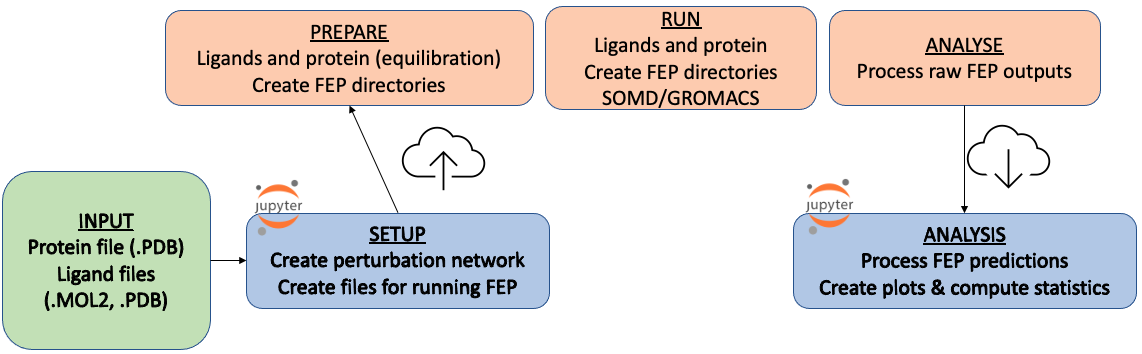
\includegraphics[width=\linewidth]{04_fep/inputs/tut_imgs/fep_pipeline.png}
\caption{figure description.}
\label{label_of_figure}
\end{figure}

%% REFER TO FIGURES LIKE THIS:
\ref{label_of_figure}